\documentclass[12pt]{article}

% pacchetti 
\usepackage[italian]{babel}
\usepackage{graphicx}
\usepackage{svg}
\usepackage{url}

\usepackage{geometry}
 \geometry{
 a4paper,
 left=25mm,
 top=25mm,
 }
 
\usepackage{hyperref}
\hypersetup{
    colorlinks,
    citecolor=blue,
    filecolor=blue,
    linkcolor=blue,
    urlcolor=blue
}

\usepackage{tikz}
\def\checkmark{\tikz\fill[scale=0.4](0,.35) -- (.25,0) -- (1,.7) -- (.25,.15) -- cycle;} 

%bibliography
\usepackage[sorting=none, isbn=false, eprint=false]{biblatex}
\addbibresource{bibliography.bib}


% set images path 
\graphicspath{ {./images/} }
% specify different fonts for headings 

\usepackage{color}

\definecolor{dkgreen}{rgb}{0,0.6,0}
\definecolor{mauve}{rgb}{0.58,0,0.82}
\definecolor{chromeyellow}{rgb}{1.0, 0.65, 0.0}

%______________Team's comments______________%

\newcommand{\edoardo}[1]{{\bf \color{red} Edoardo: #1 }}
\newcommand{\andrea}[1]{{\bf \color{mauve} Andrea: #1 }}
\newcommand{\davide}[1]{{\bf \color{chromeyellow} Davide: #1 }}
\newcommand{\piaget}[1]{{\bf \color{dkgreen} Piaget: #1 }}

%______________________Listing________________________%

\usepackage{listings}

\definecolor{codegreen}{rgb}{0,0.6,0}
\definecolor{codegray}{rgb}{0.5,0.5,0.5}
\definecolor{codepurple}{rgb}{0.58,0,0.82}
\definecolor{backcolour}{rgb}{0.95,0.95,0.92}

\lstdefinestyle{mystyle}{
    language=Java,
    aboveskip=5mm,
    belowskip=5mm,
    columns=flexible,
    backgroundcolor=\color{backcolour},   
    commentstyle=\color{codegreen},
    keywordstyle=\color{magenta},
    numberstyle=\tiny\color{codegray},
    stringstyle=\color{codepurple},
    basicstyle=\ttfamily\footnotesize,
    breakatwhitespace=false,         
    breaklines=true,                 
    captionpos=t,                    
    keepspaces=true,                 
    numbers=left,                    
    numbersep=5pt,                  
    showspaces=false,                
    showstringspaces=false,
    showtabs=false,                  
    tabsize=2
}

\lstset{style=mystyle}




\begin{document}
% pagina iniziale

\begin{figure}
    \centering
    
\includegraphics[width=0.2\linewidth]{images/unito_logo.jpg}
\end{figure}

\begin{center}
    \vspace{5ex}
    {\huge \textbf{Esame di Design Patterns}}
    \vspace{5ex}
\end{center}

\begin{center}
    Andrea Balbo Mossetto \\
    Davide Marietti \\
    Piaget Bouaka \\
    Edoardo Pastori
\end{center}

\vspace{10ex}

\begin{center}

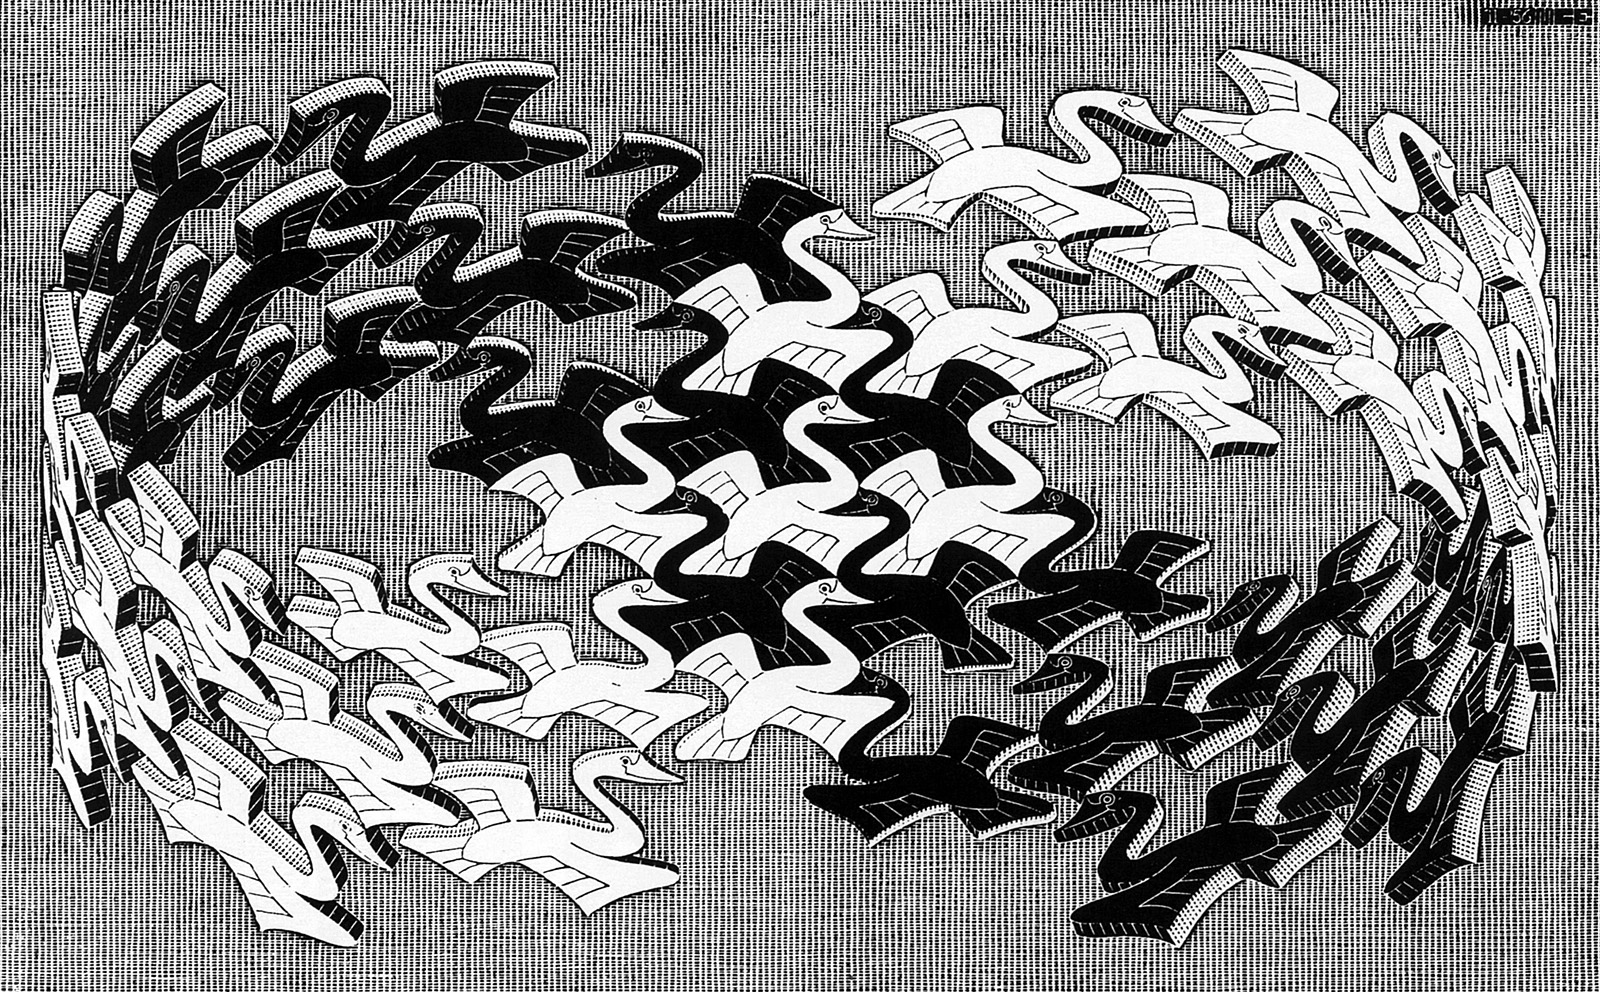
\includegraphics[scale=2]{design_pattern.jpeg}

\vspace{20ex}

Master IT Full Stack Design and Development, a.a. 2022/2023

\end{center}


\newpage

\tableofcontents

%\newpage
%\listoffigures

\newpage

\abstract{}
In questo documento \'e proposto il lavoro relativo alla realizzazione di un \textit{e-shop} di abbigliamento \textit{innovativo}. Una definizione pi\'u precisa di questo aggettivo ha richiesto una fase convergente, legata alla presa di coscienza delle caratteristiche proprie di quelli che sarebbero diventati i nostri \textit{competitors}, nonch\'e una fase divergente, attraverso la quale ci siamo soffermati sulle caratteristiche in linea con quella che iniziava a delinearsi con la nostra definizione di \textit{innovativo} mutuate da domini non appartenenti al mondo dell'\textit{e-shop} e dell'abbigliamento. 
\\
\davide{[TODO] Da AMPLIARE completandolo.}

\newpage

% capitoli 
\section{Elicitazione dei requisiti}
Questo capitolo raccoglie i requisiti che andranno poi analizzati, modellati e specificati nella fase di \textbf{Analisi dei Requisiti}. 
\\
\\
I problemi comuni da evitare in questa fase iniziale, per uno sviluppo florido del progetto, riferiscono a 3 domini principali:
\begin{enumerate}
	\item \textbf{Scopo}: i requisiti devono riflettere i bisogni del cliente
	\item \textbf{Comprensione}: \'e necessaria una buona comunicazione tra clienti, sviluppatori ed utenti per portare sul pratico i bisogni del cliente, che rifletteranno quelli degli utenti a cui vuole rivolgersi
	\item \textbf{Volatilit\'a}: i requisiti possono cambiare, non essere completi all'inizio dello sviluppo ed evolvere nel tempo; \'e quindi necessario definirli con quanta pi\'u perizia possibile in questa fase del processo
\end{enumerate}

\davide{\textbf{[TODO]} Ampliare la parte sugli strumenti utilizzati per fare la requirement elicitation.}

Si rende quindi necessaria una stretta comunicazione con il cliente, rappresentato dalla Professoressa Bono, per giungere ad un insieme di conoscenze che permetta di superare i problemi esposti poco sopra. \\
La strategia adottata \'e quella dell'\textbf{intervista}, alla quale siamo giunti dopo un \textit{brainstorming} che ci ha visto partecipi in un'iniziale definizione delle caratteristiche che, a nostro parere, dovrebbero appartenere ad un \textit{e-shop innovativo}.

Le nostre riflessioni sono sintetizzate nella sezione successiva. 

\subsection{Analisi di mercato e idee di prodotto} 
In questa fase abbiamo tratteggiato i contorni, ancora sfumati, dell'applicazione. Servono più informazioni possibili per avere una \textbf{visione ampia del mercato} in cui il prodotto richiesto si collocherà, ma anche idee originali a cui ispirarsi, che non devono necessariamente venire dal mondo dell'abbigliamento. Bisogna guardare al di là del {\em main stream}, l'applicazione dovrebbe creare l'effetto wow!
Un'analisi di mercato approfondita ci ha permesso di individuare e confrontare le caratteristiche dei competitors e di pensare a possibili \textbf{soluzioni innovative} non ancora presenti sul mercato da proporre al committente.
\\
\davide{[TODO] Da ampliare e aggiungere TABELLA della comparativa con i competitors trovati cercando su internet. Ampliando, fare riferimento alla tabella.}

\begin{table}[h!]
\centering
\begin{tabular}{|c c c c c c|} 
 \hline
  & Sost. Ambientale & Sost. Sociale & Eco. Circolare & Linea Green & ... \rule[-2ex]{0pt}{6ex} \\
 \hline\hline
 YOOX & & & & & ... \rule[1ex]{0pt}{3ex}\\ 
 Net a Porter & & & & & ... \rule[1ex]{0pt}{3ex}\\
 Patagonia & \checkmark & \checkmark & & & \rule[1ex]{0pt}{3ex}\\
 SSENSE & & & & & \rule[1ex]{0pt}{3ex}\\
 Garment Workshop & \checkmark & & & & ... \rule[1ex]{0pt}{3ex}\\
 ... & & & & & ... \rule[-2ex]{0pt}{6ex}\\
 \hline
\end{tabular}
\caption{Tabella comparativa risultato dell'analisi di mercato. \davide{[TODO] Completare la tabella con i dati presenti sul file world ed editarla stilisticamente.}}
\label{table:analisi_mercato}
\end{table}

 
 
\subsection{L'intervista}

L'intervista al committente dell'applicazione segue l'iniziale fase di analisi di mercato e di individualizzazione di possibili sviluppi innovativi, la quale è stata essenziale per \textbf{strutturare l'intervista} e raccogliere le idee innovative da proporre al committente. Le informazione raccolte nell'intervista serviranno a definire chiaramente i contorni dell'applicazione e a selezionare i moduli innovativi da sviluppare. L'intervista è stata strutturata nel seguente forma a macro blocchi:

\davide{[TODO] Ampliare e abbellire le risposte della prof alle domande fatte a lezione. Io ho scritto quello che mi ricordavo, Edoardo, completa con quello che ti ricordi tu.}

\textbf{Chi:} in questa prima fase conoscitiva abbiamo voluto inquadrare meglio la figura del committente. Abbiamo chiesto:
\begin{itemize}
    \item {\em Descrizione dell'azienda. La sua dimensione e il fatturato? La localizzazione?} Il cliente è l'{\em Atelier Splendor}, una micro azienda di abbigliamento. Possiede una sartoria interna che produce vestiti con il proprio marchio. Attualmente impiega due sarte. Il fatturato non è stato comunicato. L'azienda ha una sola sede nel centro storico di Torino.
    \item {\em Chi sono gli utenti? Target utente finale è basso/medio/alto spandente? giovane/meno giovane, con quali valori e cultura)? Il target futuro deve rimane lo stesso?} Il target di clienti attuale è alto spendente ed è concentrato nella fasci di età tra i 35 e i 60 anni. Il cliente tipo è colto e molto sensibile ai valori della sostenibilità. In futuro l'azienda desidera mantenere il proprio target, estendendolo ulteriormente verso una fascia di età più giovane, ma sempre alto spendente (Quindi max 25 anni, da quando si inizia ad avere uno stipendio).  
    \item {\em Su quale mercato opera attualmente? Su quale mercato punta a operare in futuro?} Attualmente opera sul mercato locale, tipicamente circoscritto alla provincia di Torino. La finalità dell'applicazione del negozio online è anche quella di far varcare i confini ai prodotti dell'{\em Atelier Splendor} e di puntare con la giusta consapevolezza al mercato internazionale.
\end{itemize}

\textbf{Che cosa}: in questa seconda fase sempre conoscitiva abbiamo voluto inquadrare meglio le esigenze del committente. Abbiamo voluto carpire qual'è la sua idea di applicazione finale e le caratteristiche salienti che dovrebbero essere imprescindibili. La raccolta di queste informazioni è stata essenziale per capire il contesto in cui si opera e per selezionare le idee innovative (inizialmente pensate nella fase di analisi di mercato) da proporre al cliente.
\begin{itemize}
    \item {\em Cosa motiva lei e gli stakeholders? Quali sono i vostri valori? In particolare, quali le aspettative in merito al prodotto?} Non vogliamo l’{\em hype} ({\em e.g.} Supreme, vuole la sostanza e la consapevolezza (per se stessi e per l'ambiente). Il cliente dell'{\em Atelier Splendor} sceglie un vestito per dire chi è, non lascia decidere alla massa cosa dovrebbe indossare, chi dovrebbe essere. Questa azienda promuove la cultura dello slow e della consapevolezza. Rifiutando i canoni della GDO, vuole sbarcare sul mercato online seguendo il proprio paradigma.
    \item {\em Quali sono gli obiettivi dell’azienda? L’obiettivo principale, gli obiettivi a breve, medio e lungo termine (possibilmente in ordine di importanza)?} L'obiettivo a breve termine è di espandersi attraverso l'apertura di un negozio online. L'obiettivo a medio termine è di farsi conoscere sul mercato.
    \item {\em Quali sono i criteri di successo del prodotto? Quali potrebbero essere gli indicatori da monitorare durante il progetto e quale sarebbe un indicatore chiave per stabilire che l'applicazione ha avuto successo?} L'indicatore chiave, tornasole del successo, sarebbe l'impiego di nuovo personale nella sartoria, almeno due nuove sarte.
\end{itemize}

\textbf{Quando}: in questa terza fase sempre conoscitiva abbiamo voluto inquadrare meglio le tempistiche relative alla finalizzazione del progetto. Lo scopo di queste domande è di carpire quali/quante idee innovative selezione nella (successiva) fase di brainstorming con il cliente. Il tempo a disposizione determina una selezione che andrà discussa con il cliente e una ripartizione delle idee di valore in moduli ``core", moduli ``pilota" e moduli non presi in considerazione in questa fase.
\begin{itemize}
    \item {\em Quando l'applicazione dovrebbe uscire sul mercato?}
    \\
    ...
\end{itemize}

\textbf{Brainstorming}: in questa fase abbiamo proposto idee al cliente sulla base di quanto raccolto nelle domande precedenti dell'intervista. Le idee proposte sono state avvalorate da una precedente analisi di mercato e dalle conoscenza del nostro esperto di dominio. L'insieme delle idee raccolte è poi stato ridiscusso con il cliente e suddiviso in gruppi, come presente nei risultati.
\\

\subsection{I risultati}

I risultati dell'intervista possono essere suddivisi in tre macro gruppi.
Le idee che per motivi strategici o di tempo non vengono ulteriormente sviluppate sono finite nel gruppo dei moduli attualmente non presi in considerazione, e di seguito non presentati.

La progettazione e lo sviluppo completo dei \textbf{moduli ``core"}, strategici per raggiungere gli obiettivi del cliente e contribuire al tasso di innovazione dell'applicazione. L'investimento del cliente e le forze in gioco del team rendono questi obiettivi realistici e realizzabili.
\\
\piaget{\textbf{[NOTA]} Qui ci sono i moduli da associare a qualche design pattern.}
\begin{itemize}
    \item {\em ``Popup Stores"}: non molti negozi fisici, ma spot stores temporanei, localizzati dove sono concentrati la maggior parte dei clienti. La creazione di una rete di aziende amiche che condividono gli stessi ideali di sostenibilità permette numerosi vantaggi. {\em Atelier Splendor} ospiterà virtualmente i capi di queste aziende nel suo futuro negozio virtuale, queste aziende ospiteranno mostre temporanee dei nostri capi nei loro negozi fisici. La scelta delle città in cui organizzare le mostre verrà suggerita dai dati raccolti.
    \item {\em ``Vestirsi con la realtà aumentata"}: Algoritmo di realtà aumentata stile Ikea che consente di vestirsi virtualmente per provare i vestiti e trovare la propria taglia. Ciò sorride all'ambiente e fa l'occhiolino al consumatore consapevole perché permetterà di ridurre il numero dei resi. Cliente soddisfatto e ambiente pure. 
    \item {\em ``Magazzino Snello"}: rivedere il data model del magazzino da integrare in un data base pinco pallino su cui poggerà la nostra applicazione. Questo consentirà agli impiegati dell'azienda di loggarsi come tali e di monitorare meglio le risorse e i flussi di magazzino, abbattendo i costi generati dalla merce invenduta.
    \item {\em ``Go Circular!"}: sezione dell'applicazione dedicata ai vestiti usati che viene alimentata dai vestiti creati dall'atelier e dati indietro dai clienti in cambio di un vaucher da spendere sui vestiti nuovi confezionati dall'atelier. In questo modo il negozio ospiterà sì brand diversi e sostenibili, ma cerchiamo di favorire l'acquisto di abiti con il nostro brand. Questa politica, che sorride all'ambiente, sorride anche all'espansione della sartoria e all'assunzione di nuovo personale. Inoltre, gli abiti dati indietro spesso necessiteranno una sistemata da parte delle nostre sarte prima di essere caricato online.
    
\end{itemize}

La progettazione e lo sviluppo almeno parziale dei \textbf{moduli ``pilota"}, strategici ai fine del marketing e strategici in futuro, non appena verranno raggiunti gli obiettivi prefissati più importanti (assunzioni di nuove sarte e aumento del numero di clienti). Le condizioni attuali non consentono lo sviluppo completo di questi moduli. Lo sviluppo futuro di questi moduli consentirà una fruttuosa e duratura collaborazione con l'{\em Atelier Splendor}.
\begin{itemize}
    \item {\em ``Algoritmo di consiglio all'acquisto human-driven"}: l'output dell'algoritmo non viene direttamente fornito al cliente, ma è mediato dall'essere umano, nello specifico un esperto di moda, che spiega il perché di questo consiglio di acquisto.
    \item {\em ``Marketing"}: Nell'ambito del marketing, prodotti mirati saranno associati a un link di un contento Tiktok di un influencer che starà indossando quel vestito. Questo per ampliare il target verso una fascia più giovane.
    \item {\em ``Sartoria dedicata e confezionamento su misura"}: la sartoria interna potrà essere ulteriormente allargata introducendo due nuovi servizi al cliente. Primo, i vestiti che necessiteranno di manutenzione (orli, pence, sostituzione cerniere, rattoppi, ...) potranno essere spediti alla sede centrale per essere aggiustati. Due, la sartoria offrirà la possibilità di avere abiti confezionati su misura.
\end{itemize}


\section{Analisi dei requisiti}

In questa sezione riportiamo i requisiti che la nostra applicazione dovrà rispettare e seguire nello sviluppo.

\davide{\textbf{[TODO]} Ampliare questa parte introduttiva.}

\subsection{Attori, obiettivi e Casi d'Uso}
\label{subsec:UC}

L'applicazione e tutto il sistema che traduce deve essere pensata per essere sfruttata da una serie di attori, umani o meno, che, con le loro attivit\'a, determinano come essa sar\'a sviluppata. Possiamo classificare gli attori nella tassonomia seguente:
\begin{itemize}
    \item Gli \textbf{attori principali} sono quelli che utilizzano direttamente l’applicazione per uno specifico use case (sono i fruitori dell’app, e.g. un cliente, un impiegato).
    \item Gli \textbf{attori secondari} sono sistemi esterni (tipicamente software) che integriamo all’interno dell’app (sono API che inseriamo per implementare il tutto e su cui non abbiamo controllo).
    \item Gli \textbf{attori fuori scena} sono entità che non usano direttamente l’app, ma che ne possono trarre benefici o ci danno dei vincoli da rispettare (l’università è l’attore fuori scena che beneficia di Moodle, la legge con il GDPR).
\end{itemize}

I Casi d'Uso, invece, descrivono i possibili scenari di utilizzo dell'applicazione, il macro-contesto all'interno del quale si muovono gli attori di cui sopra. Una comune rappresentazione grafica di un Caso d'Uso (od \textbf{UC}) \'e ravvisabile nell'{\em UC diagram}, ovvero un'\textit{interfaccia} astratta della nostra applicazione (cfr. fig. \ref{fig:UC_diagram}, p.\pageref{fig:UC_diagram}).
\\
\\
La definizione degli attori deriva da quella degli UC, pertanto ci aggiungiamo ad elencare quelli che saranno di nostro interesse progettuale:
\begin{itemize}
    \item Acquisto di capi di vestiario online (\textit{UC1})
    \item Accesso al magazzino snello (\textit{UC2})
    \item Aggiornamento dei clienti rispetto all'installazione temporanea di Pop-Up store (\textit{UC3})
\end{itemize}

A questo punto possiamo enunciare gli attori, a pi\'u livelli, che entreranno in contatto con gli UC che abbiamo appena definito. In particolare:
\begin{itemize}
	\item \textbf{UC1}
		\begin{itemize}
		\item Principali: Cliente che vuole acquistare - Dipendente che monitora acquisti 
		\item Secondari: Metodi di pagamento
		\item Fuori scena: Compagnia di trasporti 
		\end{itemize}
	\item \textbf{UC2}
		\begin{itemize}
		\item Principali: Cliente nella sua forma di avatar - Dipendente sarto che gestisce il proprio lavoro rispetto al traffico degli avatar 
		\item Secondari: Algoritmo che coadiuva i dipendenti nella gestione del magazzino
		\item Fuori scena: Fornitori di materie prime 
		\end{itemize}
	\item \textbf{UC3}
		\begin{itemize}
		\item Principali: Cliente che vuole essere aggiornato rispetto alle attivit\'a della Compagnia 
		\item Secondari: Database collegato a software tramite API per gestire informazioni di contatto dei clienti interessati alla newsletter 
		\item Fuori scena: GDPR
		\end{itemize}
\end{itemize}

\subsection{Requisiti}

Con \textit{requisiti} intendiamo caratteristiche del sistema, da un punto di vista puramente logico o da un punto di vista tecnico. Pi\'u nello specifico, distinguiamo: 
\begin{itemize}
	\item \textbf{requisiti funzionali}, che riguardano ciò che il sistema fa e sono i moduli da implementare o integrare per lo sviluppo dell’applicazione;
	\item \textbf{requisiti non funzionali}, che riguardano come \'e fatto il sistema (riferendoci ad esempi quali i tools che vengono utilizzati per la sua realizzazione, il linguaggio di programmazione con cui \'e scritto, il database a cui si appoggia, ...)
\end{itemize}

Descriviamo quindi i requisiti che abbiamo intercettato relativamente agli UC individuati nella sezione precedente: 
\begin{itemize}
	\item UC1
		\begin{itemize}
		\item funzionali: voglio permettere all'utente di accedere al mio sito web e alla mia applicazione, visualizzare l'elenco degli articoli a mia disposizione, fargli scegliere quelli che pi\'u lo aggradano, inserirli nel carrello, pagare e completare l'ordine. Voglio permettere al dipendente di visualizzare gli ordini 
		\item non funzionali: tools Java (pattern decorator + strategy), html+javascript+css (front-end), Oracle. 
		\end{itemize}
	\item UC2
		\begin{itemize}
		\item funzionali: voglio permettere all'utente di gestirsi (eventualmente) l'avatar, tramite cui provera' le diverse combinazioni di capi. I dati immagazzinati serviranno al sarto per una gestione pi\'u lean del magazzino (vedi anche ordini con i fornitori di materie prime)
		\item non funzionali: Oracle, Java (pattern Composite), Three-js (libreria js sul browser per realt\'a aumentata)/ webGL (grafica 3D)
		\end{itemize}
	\item UC3
		\begin{itemize}
		\item funzionali: voglio permettere ai miei "iscritti" di ricevere info riguardanti i prossimi eventi pop-up store nella zona geografica di competenza 
		\item non funzionali: Oracle, Java (pattern Observer), client mail, API di geolocalizzazione
		\end{itemize}
\end{itemize}


\vspace{1em}
\begin{figure}[ht]
  \centering
   \makebox[\textwidth][c]{\includesvg[width= 1.1\linewidth]{UC_diagram.svg}}
  \caption{\small Esempio di UC diagram relativo all'applicazione del negozio online. All'interno delle {\em system boundaries} sono posizionati i casi d'uso esaminati in questa sezione. Gli attori principali (azzurro), quelli secondari (verde) e quelli fuori scena (giallo) sono rappresentati dalle figure al di fuori del {\em system} e sono collegati ai relativi casi d'uso. Una più approfondita analisi del diagramma è presentata in sezione \ref{subsec:UC}}
  \label{fig:UC_diagram}
\end{figure}


\subsection{Glossario degli attori}

Viene fornito al lettore un glossario dei termini tecnici utilizzati nelle sezioni precedenti:
\begin{itemize}
	\item API: \textit{``le API sono meccanismi che consentono a due componenti software di comunicare tra loro usando una serie di definizioni e protocolli. Ad esempio, il sistema software dell'ufficio metereologico contiene dati metereologici giornalieri. L'app del meteo sul cellulare ``parla'' con questo sistema tramite API e mostra gli aggiornamenti metereologici quotidiani sul telefono''} (cfr. \cite{bworld})
	\item Client mail: un programma che permette di gestire il servizio di posta elettronica 
	\item Database: \textit{un database \'e una collezione organizzata e strutturata di dati. Il database \'e controllato da un Database Management System (DMBS), che funge da interfaccia tra l'utente che vuole avere accesso ai dati e il pc su cui questi dati sono salvati} (cfr. \cite{database}); un celebre esempio di DBMS e' Oracle. 
	\item Libreria: insieme di funzioni e strutture dati che permette allo sviluppatore di avere a propria disposizione codice gi\'a pronto alle proprie necessit\'a
	\item Linguaggio di marcatura: insieme di regole che definiscono e strutturano l'impaginazione di un testo. Faremo in particolare ricorso ad \textit{HTML} e \textit{CSS}. La stesura di codice in questi linguaggi definir\'a ci\'o che gli utenti vedranno tramite interfaccia
	\item Linguaggio di programmazione: linguaggio formale che specifica un insieme di istruzioni che vorranno interpretate e/o compilate dal computer, restituendo dei dati in uscita. Ci avvaliamo di \textit{Javascript} e \textit{Java}
	\item Pattern (\textit{Design Pattern}): modello logico a cui si ricorre per proporre una soluzione ad un problema che riguarda l'architettura e la progettazione del programma. 
\end{itemize}


\section{Il documento di vision}

\davide{\textbf{TODO} Da elaborare!}


\section{Design Patterns utilizzati}

Un {\em pattern} è una soluzione generale ad un problema ricorrente, che va opportunamente adattato al problema in esame (cfr.\cite{gof_riferimento}, p.12). Un Pattern può essere riassunto in: problema, soluzione, pro e contro della soluzione ed esempi d’uso. I Design pattern visti a lezione sono i \textbf{GoF Design Pattern} e permettono di sfruttare al massimo le caratteristiche object oriented di Java. Essi costituiscono di fatto una mappa per scrivere codice Java \cite{gof_sunt}.

In questa sezione riportiamo sottoforma di micro-prototipi le implementazioni dei design pattern applicati ai casi d'uso della nostra applicazione.

\begin{itemize}
    \item Con riferimento al caso d'uso dell'acquisto di capi di vestiario online, un dipendente dell'atelier può anche essere un cliente e utilizzare l'applicazione con due scopi differenti: per controllare gli ordini da evadere o per acquistare capi sullo store online.
    Abbiamo quindi pensato di modellare la figura del {\em dipendente-cliente} tramite due pattern alternativi: il \textbf{pattern Decorator} (cfr.\cite{gof_riferimento}, p.196) e il \textbf{pattern Strategy} (cfr.\cite{gof_riferimento}, p.349). Ciò ci ha permesso di confrontare e discutere i vantaggi/svantaggi di questi due patterns.
    \item Con riferimento al caso d'uso dell'accesso al magazzino snello, possiamo ricollegarci al modulo sull'approccio human-driven per implementare il \textbf{pattern Composite} (cfr.\cite{gof_riferimento}, p.183). Lato tecnico usiamo il pattern composite. Lato umano, i sottoinsiemi generati dal composite verranno filtrati dall'umano esperto.
    Alternativamente, il pattern composite potrebbe essere applicato semplicemente al caso d'uso dell'accedere al magazzino snello con riferimento al modulo del {\em magazzino snello}.
    \item Con riferimento al caso d'uso dell'aggiornare i clienti rispetto all'installazione di Pop-Up stores temporanei, l’idea di allestire una newsletter ci ha indirizzati nell'implementazione del \textbf{pattern Observer} (cfr.\cite{gof_riferimento}, p.326).
\end{itemize}


\andrea{\textbf{[NOTA]} Obbligatorio il design pattern {\em Composite} con almeno tre livelli che restituisca, e.g. le componenti di abbigliamento che formano l'outfit. Più siamo fantasiosi nel trovare un'applicazione tra le nostre idee, meglio verrà valutato.}


\davide{Materiale da citare: \cite{gof_riferimento}, \cite{up-riferimento}, \cite{uml_riferimento}, \cite{elicitation_tools}, \cite{gof_sunt}, \cite{github}.}


\subsection{Pattern Decorator}

Il {\em pattern Decorator}, noto anche come {\em Wrapper}, permette di aggiungere dinamicamente responsabilità addizionali ad un oggetto individuale. In questo modo si possono estendere le funzionalità di oggetti particolari senza coinvolgere intere classi (cfr.\cite{gof_sunt}, p.65).
\\
\\
Un modo per aggiungere responsabilità ad un oggetto potrebbe essere tramite la semplice {\em ereditarietà}. Ciò consente una certa flessibilità, tuttavia rimane una certa staticità dovuta al fatto che il client non può controllare quanto e come aggiungere tale proprietà all'oggetto.
Un approccio più flessibile è dato dall'includere l'oggetto che si vuole decorate in una {\em wrapper classes} (il {\em Decorator}) che aggiunge la nuova responsabilità voluta. Gli oggetti decorati assieme al Decorator devono sottostare a una interfaccia comune, che rende la sua presenza {\em trasparente} e permette all’applicazione di continuare ad interagire con gli oggetti decorati \cite{gof_sunt}. Tale proprietà di trasparenza rende iterativa e potenzialmente illimitata l'applicazione di responsabilità aggiuntive tramite nuovi Decorators.
La proprietà di trasparenza permette inoltre ai decorators di apparire ovunque l'oggetto da decorare possa apparire, in modo che i clients non siano in grado di distinguere un oggetto decorato da uno che non lo sia \cite{gof_riferimento}.
\\
\\
Un esempio illuminante di possibile utilizzo ci è proposto dalla {\em Gang of Four} (cfr.\cite{gof_riferimento}, p.197):
Supponiamo di avere un oggetto TextView che mostra del testo in una finestra. Di default, la TextView non ha scroll bar, perchè non sempre ne abbiamo bisogno. Quando necessario possiamo ``decorare'' la TextView con una scroll bar. Supponiamo di volere anche un bordo più spesso attorno alla finestra. Possiamo ``decorare'' l'oggetto TextView anche con quello e con tutte le altre caratteristiche aggiuntive fino a ottenere il risultato voluto.

Con riferimento invece al caso d'uso dell'acquisto di un abito sull'applicazione, si pensi ad un modello di oggetti che rappresenti i dipendenti dell'Atelier Splendor. Un impiegato può essere un cliente interessato a comprare un abito sulla piattaforma. Nasce così l'esigenza di modellare la figura dell'\textbf{dipendente-cliente}, il quale in aggiunta alle operazioni definite per i dipendenti, definisce anche quelle relative ai clienti.
\\
\\
Il pattern Decorator ha i seguenti \textbf{vantaggi} evidenti:
\begin{itemize}
    \item Il pattern Decorator è più \textbf{flessibile} dell'ereditarietà statica (multipla). Con il Decorator le responsabilità possono essere infatti aggiunte/tolte dinamicamente a {\em run time}, semplicemente attaccando o staccando il Decorator. Mentre utilizzando l'ereditarietà servirebbe creare una nuova classe per ciascuna nuova responsabilità addizionale, con il conseguente proliferare di classi che aggiungo complessità al sistema. Inoltre, con il Decorator avrei il vantaggio di poter combinare liberamente tra loro le varie responsabilità. Infine, il Decorator rende più semplice e meno prono ad erri l'aggiungere più volte una stessa proprietà a un dato oggetto (e.g. nel caso della TextView, di aggiungere due volte il bordo) \cite{gof_riferimento}.
    \item Evita che classi ricche di caratteristiche scalino la gerarchia. Il Decorator offre infatti un \textbf{approccio ``pay-as-you-go''} all'aggiunta di responsabilità: invece di cercare di gestire tutte le caratteristiche di un oggetto in un'unica classe grande e complessa, possiamo definire una classe semplice e aggiungerci le caratteristiche in modo \textbf{incrementale} con gli oggetti Decorator. Le funzionalità vengono composte da pezzi piccoli e semplici.
    Come risultato un'applicazione non deve ``pagare'' per caratteristiche che non usa \cite{gof_riferimento}.
    Questo approccio semplifica anche la definizione di nuove caratteristiche che non erano state pensate o incluse in partenza, evitando che l'estensione di una classe complessa possa esporre dettagli non connessi alle responsabilità che vogliamo aggiungere.
\end{itemize}
Mentre gli \textbf{svantaggi} più evidenti sono:
\begin{itemize}
    \item Un Decorator e i suoi {\em component} \textbf{non sono identici (==)}. Esso si comporta come un ``contenitore trasparente'', ma da un punto di vista dell'identità tra oggetti, un oggetto decorato non è uguale all'oggetto stesso non decorato. Quindi, non bisogna fare affidamento sull'identità tra oggetti (==) quando si usa questo pattern \cite{gof_sunt}.
    \item Questo pattern genera tanti ``piccoli'' oggetti simili tra di loro. Tali oggetti differiscono solo dal modo in cui sono interconnessi, non dalla classe o dal valore delle loro variabili. Seppur semplici da customizzare per chi li ha creati, risultano \textbf{difficili da comprendere e debuggare} da terzi \cite{gof_riferimento}.
\end{itemize}

Per implementare il patter Decorator abbiamo bisogno di (cfr.\cite{gof_sunt}, p.65):
\begin{itemize}
    \item Un {\em Component} ({\tt User}): definisce l'interfaccia per gli oggetti a cui verranno aggiunte proprietà in modo dinamico.
    \item Un {\em ConcreteComponent} ({\tt UtenteBase}): definisce l'oggeto su cui verranno dinamicamente aggiunte le proprietà.
    \item Un {\em Decorator} ({\tt Ruolo}): mantine una referenza al {\em Component} e definisce un'interfaccia conforme a quella del {\em Component}.
    \item Un o più {\em ConcreteDecorator} ({\tt Dipendente, Cliente}): aggiunce le responsabilità al {\em Component}.
\end{itemize}


\lstinputlisting[label={list:esempio}, caption={\small ClienteDipendente.java -- Implementazione del pattern Decorator nel caso d'uso dell'acquisto online.}]
{code/ClienteDipendente.java}


\subsection{Pattern Strategy}

Il {\em pattern Strategy} serve a definire una famiglia di algoritmi simili tra loro e dunque \textbf{intercambiabili}. In particolare, è tipica della situazione in cui vogliamo isolare l’algoritmo che svolge un certo compito, per farlo variare in modo indipendente dal resto dell’implementazione della classe.

Questo pattern suggerisce l’incapsulamento della logica di ogni
particolare algoritmo, in apposite classi, dette {\em ConcreteStrategy}, le quali implementano l’interfaccia che consente agli oggetti di interagire con loro. Questa interfaccia deve fornire un accesso efficiente ai dati del Context, richiesti da ogni ConcreteStrategy, e viceversa \cite{gof_sunt}.


\subsection{Pattern Composite}
Questo pattern ci consente di construire una gerarchie di oggetti composti. Gli oggetti composti possono essere formati da oggetti singoli, oppure da altri oggetti composti. è utile nei casi in cui si vuole rappresentare gerarchie di oggetti tutto-parte, essere in grado di ignorare le differenze tra oggetti singoli e oggetti composti. Il fatto che Splendor mostra il desiderio di vendere articoli di altri brand abbiamo visto molto opportuno propore il composite perche nell'architectura potra aggiungere gli articoli suoi e altri brand il modo facile e molto sepatato
Il pattern viene usato nel nostro caso perché si può rappresentare il nostro magazzino come segue:

\begin{figure}
    \centering
    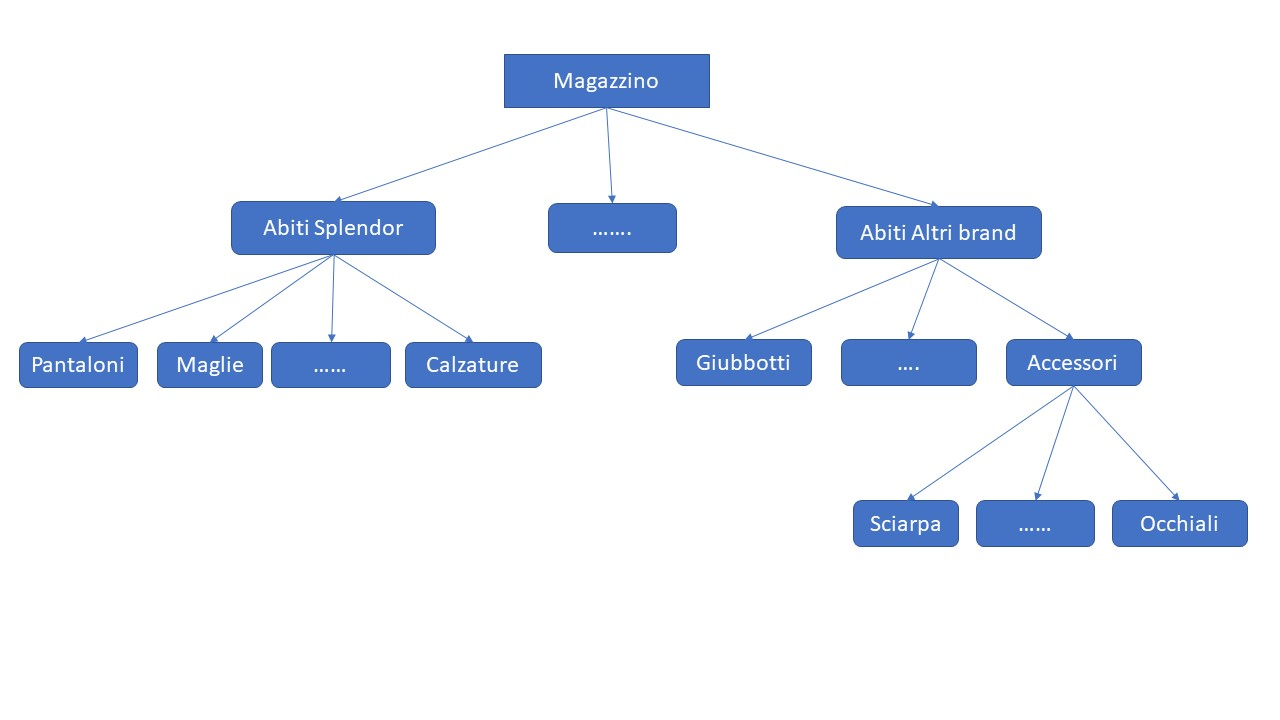
\includegraphics[width=1\linewidth]{images/Composite.jpg}
\end{figure}

Per implementare il pattern abbiamo bisogno di :
\begin{itemize}
	\item Un \textit{Item} (è una classe astratta che fornisce le operazione base del nostro magazzino/articolo)
	\item Un \textit{CompoundItem} (La classe estende Item e si comporta sia come una parte del magazzino o come il magazzino intero a secondo di come è usato)
	\item Un \textit{SaleableItem} (Questa classe è l'articolo proprio, estende Item e ha un costruttore piu completo di CompoundItem anh )
	\item Un  \textit{SaleableItemException} (Per gestire un' \textit{exception} quando l'utente prova ad aggiungere in un \textit{SaleableItem} un \textit{Item})
\end{itemize}
\begin{lstlisting}
// The Item abstract class 
public abstract class Item {
	protected String name;

	public Item(String name) {
		this.name = name;
	}

	public abstract void describe();

	public void addItem(Item c) throws SaleableItemException {
		if (this instanceof SaleableItem)
			throw new SaleableItemException();
	}

	public void removeItem(Item c) throws SaleableItemException {
		if (this instanceof SaleableItem)
			throw new SaleableItemException();
	}

	public Item getItem(int n) {
		return null;
	}
}

//CompoundItem class
public class CompoundItem extends Item {
	private ArrayList<Item> items;

	public CompoundItem(String name) {
		super(name);
		items = new ArrayList<Item>();
	}

	@Override
	public void describe() {
		System.out.println(name);
		System.out.println("\tComposed by:");
		System.out.println("\t\t{");
		items.forEach(Item::describe);
		System.out.println("}");
	}

	public void addItem(Item c) throws SaleableItemException {
		items.add(c);
	}

	public void removeItem(Item c) throws SaleableItemException {
		items.remove(c);
	}

	public Item getItem(int n) {
		if (n<0 || n>items.size()) return null;
		return (Item) items.get(n);
	}
}

// SaleableItem class
public class SaleableItem extends Item{
	private double weight;
	private String type;
	private double price;
	private String size;
	
	public SaleableItem(String name,String type, double weight, double price,String size) {
		super(name);
		this.weight = weight;
		this.price = price;
		this.type = type;
		this.size = size;
	}

	@Override
	public void describe() {
		 System.out.println( "SaleableItem: " + name  +", type: "+type +", weight: "+weight +"kg"+", price: "+price +"€" +", size:" + size); 
		
	}
 }

 // SaleableItemException class
 public class SaleableItemException extends Exception {
	public SaleableItemException() {
		super("Not supported method, you cant add Item on SaleableItem");
	}
}
\end{lstlisting}
Come detto prima, la classe \textit{CompoundItem} può rappresentare l'intero magazzino o semplicemente una parte (categoria) di alcuni articoli. La classe \textit{CompoundItem} è usata per rapprensentare tutti gli articoli di Splenldor e quelli di altri brand che il loro insieme forma tutto il magazzino che è sempre rapprensatato da la classe \textit{CompoundItem}.
\\
La classe \textit{SaleableItem} rappresenta l'articolo venduto con tutto le caratterische possibile, ogni volta che si vuole aggiungere un articolo (\textit{SaleableItem}) si chiama la \textit{addItem} sul Magazzino (\textit{CompoundItem})
\\
\textbf{NB}: Chiamando la addItem o removeItem su \textit{SaleableItem} lancierà la \textit{SaleableItemException}


\subsection{Pattern Observer}

Il pattern \textit{Observer} (noto anche come \textit{Publish-Subscribe}) \'e un pattern TIPOPATTERNEDEFINIZIONE, che "\textit{definisce una relazione uno-a-molti tra oggetti, in modo tale che, quando un oggetto cambia stato, tutti i suoi dipendenti siano notificati e aggiornati automaticamente}" (\cite{gof_riferimento}, p.326). 
\\
\\
L'adozione di questo pattern trova le sue radici nella necessit\'a di trovare una \textit{consistenza} tra oggetti appartenenti a classi che \textit{cooperano} tra loro; una soluzione che sarebbe possibile adottare sarebbe quella di rendere queste classi strettamente dipendenti le une dalle altre, ma questo ridurrebbe la loro riusabilit\'a. La \textit{Gang of Four} cita come esempio la situazione in cui una diversa rappresentazione grafica (un grafico a barre, un grafico a torta e una rappresentazione tabellare) prendano le informazioni circa i dati da rappresentare dal medesimo \textit{data object}. Queste rappresentazioni grafiche non comunicano direttamente tra loro, ma devono comportarsi come se lo potessero fare. Quindi, nel momento in cui l'utente cambia i dati, questo cambiamento deve riflettersi in tutte le rappresentazioni grafiche di cui sopra. (cfr. \cite{gof_riferimento}, p.327)
\\
\\
Questo comportamento implica quindi, accettando il fatto di non voler creare dipendenze tra questi tre oggetti, che essi vengano notificati e coerentemente aggiornati rispetto a modifiche ed aggiornamenti che si verificano per il \textit{data object} soggiacente che li popola. Il pattern Observer viene incontro a questa esigenza. 
\\
\\
Nel nostro caso specifico, essendoci immaginati, oltre allo store on-line per la vendita dei nostri prodotti, anche l'allestimento di PopUp-Store temporanei in diverse citt\'a, l'idea che gli utenti iscritti al nostro sito per effettuare acquisti potessero essere interessati ad aggiornamenti relativi alla nostra presenza fisica sul territorio, per poter toccare direttamente con mano i capi che forniamo loro, ha portato alla presa di coscienza della necessit\'a di allestire una \textit{newsletter} che li potesse aggiornare in tal senso. Essi saranno aggiornati rispetto ad informazioni chiave quali la citt\'a ed il negozio entro cui il PopUp-Store verr\'a allestito, nonch\'e gli orari. 
\\
\\
Procediamo ora con il commento del codice utilizzato. \\
L'implementazione prevede la creazione di:
\begin{itemize}
	\item Un \textit{subject} (fornisce un'interfaccia che permette di aggiungere, rimuovere e notificare gli osservatori)
	\item Un \textit{concreteSubject} (notifica gli osservatori circa i cambiamenti del proprio stato e modifica quest'ultimo all'occorrenza)
	\item Un (...n) \textit{observer} (fornisce un'interfaccia per aggiornare gli osservatori rispetto ai cambi di stato del soggetto)
	\item Un (...n) \textit{concreteObserver} (viene informato dei cambi di stato avvenuti sul concreteSubject e usa le informazioni ottenute per aggiornarsi appropriatamente rispetto ad esso)
\end{itemize}

\begin{lstlisting}
// The Subject interface 
interface Subject {
    void registerObserver(Observer o); 
    void removeObserver(Observer o); 
    void notifyObservers();
}

// The Observer interface 
interface Observer {
    void update(String location, String store, Date openingdate, Date closingdate, float openingtime, float closingtime); 
}
\end{lstlisting}

Come abbiamo detto precedentemente, queste due interfacce permettono, rispettivamente:
\begin{itemize}
	\item SI:
		\begin{itemize}
		\item aggiungere un osservatore 
		\item rimuovere un osservatore 
		\item notificare agli osservatori i cambi di stato
		\end{itemize}
	\item OI:
		\begin{itemize}
		\item essere aggiornati rispetto ai cambi di stato del soggetto
		\end{itemize}
\end{itemize}

Ribadiamo che abbiamo definito i seguenti cambi rispetto ai quali i clienti dovranno essere aggiornati:
\begin{itemize}
	\item citt\'a entro cui si svolger\'a il PopUp-Store 
	\item il negozio che lo ospiter\'a
	\item la data di apertura e quella di chiusura
	\item l'orario entro cui esso si potr\'a trovare all'interno del negozio sopracitato
\end{itemize}

Possiamo ora passare al \textit{ConcreteSubject} e al \textit{ConcreteObserver}:

\begin{lstlisting}

// The PopUpStore class is the ConcreteSubject 
class PopUpStore implements Subject {

    private List<Observer> observers; 
    private String location;
    private String store;
    private Date openingdate;
    private Date closingdate;
    private float openingtime;
    private float closingtime;

    public PopUpStore() {
    observers = new ArrayList<Observer>();
    }

    public void registerObserver(Observer o) { 
        observers.add(o);
    }

    public void removeObserver(Observer o) { 
        int i = observers.indexOf(o);
        if (i >= 0) {
            observers.remove(i); 
        }
    }

    public void notifyObservers() {
        for (Observer observer : observers) {
            observer.update(location, store, openingdate, closingdate, openingtime, closingtime); 
        }
    }

    public void measurementsChanged() { 
        notifyObservers();
    }

    public void setMeasurements(String location, String store, Date openingdate, Date closingdate, float openingtime, float closingtime) { 
        this.location = location;
        this.store = store;
        this.openingdate = openingdate;
        this.closingdate = closingdate;
        this.openingtime = openingtime;
        this.closingtime = closingtime;
        measurementsChanged(); 
    }
}


// The ConcreteObserver class
class CurrentConditionsDisplay implements Observer, DisplayElement {
    private float temperature; 
    private float humidity; 
    private Subject PopUpStore;
    
    public CurrentConditionsDisplay(Subject PopUpStore) { 
        this.PopUpStore = PopUpStore; 
        PopUpStore.registerObserver(this);
    }
    
    public void update(String location, String store, Date openingdate, Date closingdate, float openingtime, float closingtime) { 
        this.location = location;
        this.store = store;
        this.openingdate = openingdate;
        this.closingdate = closingdate;
        this.openingtime = openingtime;
        this.closingtime = closingtime;
        display();
    }
    public void display() {
    System.out.println("We look forward to seeing you at our new Pop-Up store in " + location + ", kindly hosted by  " + store + 
    ", on the following dates: " + openingdate + " - " + closingdate + ", at the following times:" + openingtime + " - " + closingtime);
    } 
}

\end{lstlisting}

Commentando questa parte di codice, notiamo che il \textit{ConcreteSubject} \'e rappresentato dal PopUp-Store che, come anticipato, pu\'o aggiungere, rimuovere e notificare gli \textit{Observers}, andando ad aggiornare i dati relativi ai campi che definiscono il nostro PopUp-Store (tramite la comunicazione diretta con l'interfaccia \textit{Observer}). Vi \'e poi un metodo per settare questi dati. 
\\
\\
Passando invece al \textit{ConcreteObserver}, vediamo che esso ha modo di registrarsi al \textit{Subject} di nostro interesse, di aggiornare le informazioni a sua disposizione relativamente ai campi che definiscono il PopUp-Store, nonch\'e averle a disposizione tramite il suo metodo \textit{display}. 
\\
\\
Il resto del codice \'e disponibile in appendice.


\newpage

%Prints the bibliography
\printbibliography


\end{document}